\documentclass{article}
\usepackage[utf8]{inputenc}
\usepackage{amsmath}
\usepackage{tcolorbox}
\usepackage{graphicx} 
\usepackage{subfigure}
\usepackage{nonfloat}
\usepackage{geometry} \geometry{a4paper, top=25mm, left=25mm, right=25mm, bottom=30mm, headsep=10mm, footskip=12mm} 
\usepackage{fancyhdr}
\usepackage{daytime}
\usepackage{hyperref}
\usepackage{blindtext}
\usepackage{enumitem}

\pagestyle{fancy}
\lhead{Jannis Hoppe}
\chead{EL2320 - Lab 2}
\rhead{\today}

\title{Project Proposal - Applied Estimation}
\author{Thomas Georg Jantos - janots@kth.se - 960508 1570\\Jannis Hoppe - jannish@kth.se - 941204 8358}
\date{December 2017}




\begin{document}
	
\maketitle
\noindent
	For our project we want to consider a robot for letter, package or tools delivery. This subject area has gotten quite some attention for drones in cities with high traffic or mobile robots for use in specific environments such as hospitals. Thus, we expect to find up-to-date research material. We want to consider the case of a campus environment, where the robot estimates its position and the current map with features such as trees. We plan on using a video dataset from Stanford University \footnote{\label{foot:1}\url{http://cvgl.stanford.edu/projects/uav_data/}}, with an environment like the one shown in figure \ref{fig:Bild1}. The video material has to be preprocessed as a first step. We could add a fictive robot to the environment moving e.g. from the bottom left to the top right corner "measuring" the distances to all the objects in its vicinity. We want to implement at least a well working SLAM method and then, if we have time, add models for the estimation of moving objects such as people, vehicles or cyclists.This way we could analyze what we have to do in order to make the studied algorithms work for (more realistic) dynamic environments. We will probably use a particle filter. An advantage of this project is, that we can work in distinct steps, in which complexity is stepwise added to the problem: first we implement the filter with a known map, then SLAM, then a dynamic environment (as well as possible in the given time).
	
	
	\begin{figure}[htbp] 
		\centering
		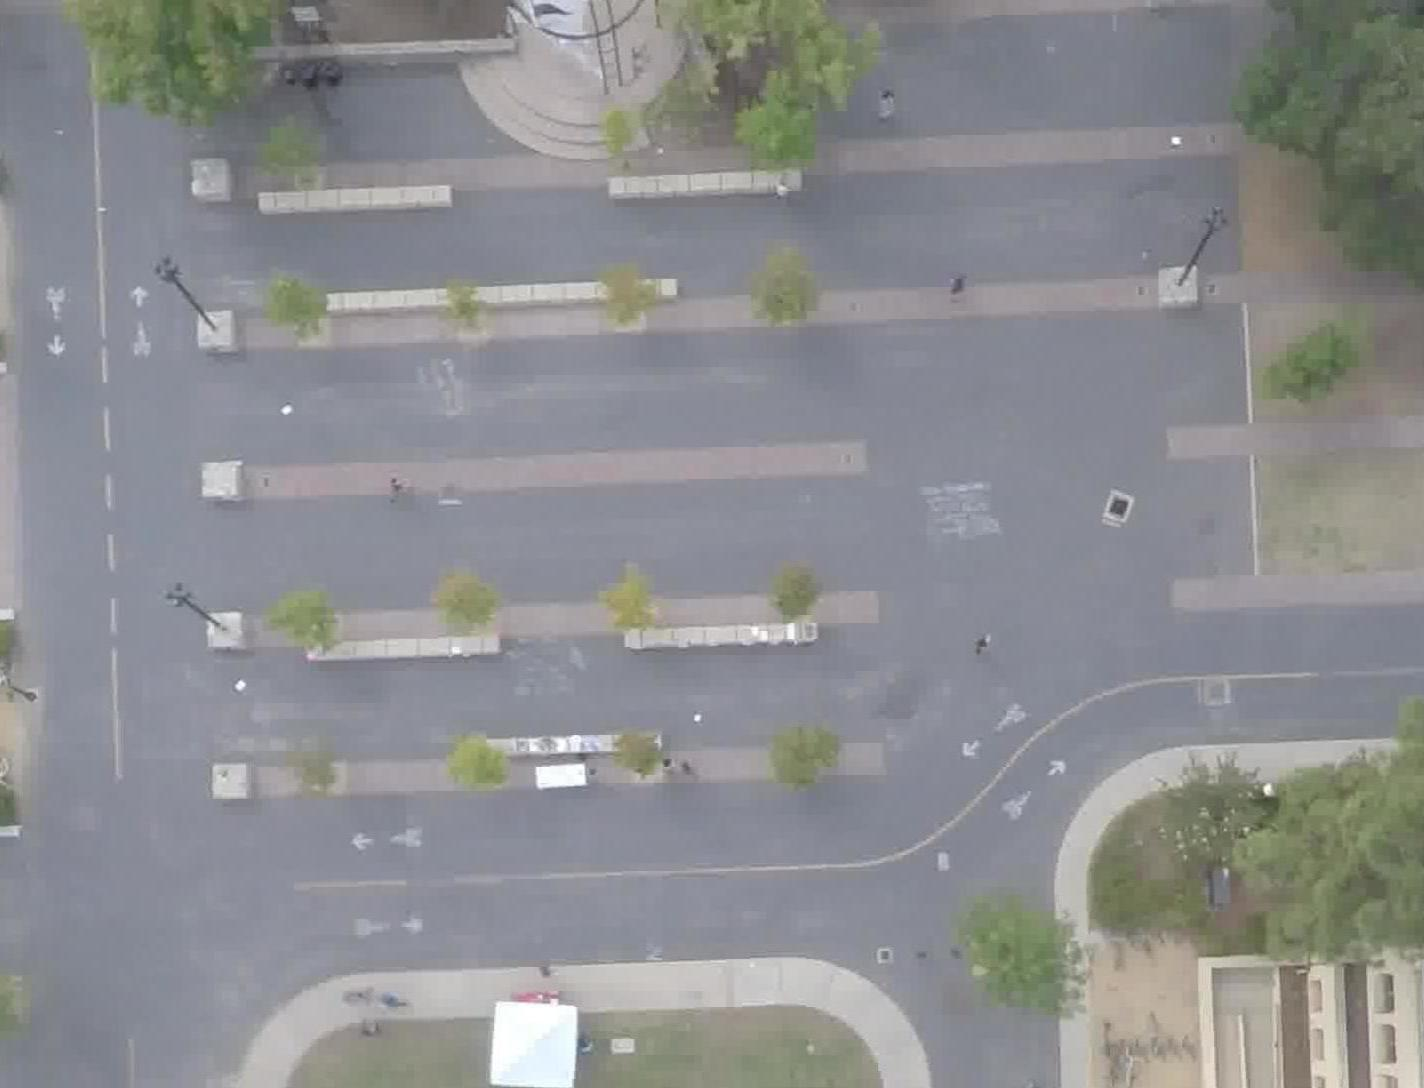
\includegraphics[width=0.7\textwidth]{reference.jpg}
		\caption{Screenshot taken from the Stanford University dataset.}
		\label{fig:Bild1}
	\end{figure}
\pagebreak

\begin{enumerate}
	
	\item Notwendige Arbeitsschritte:
\begin{itemize}
	\item inhalte für literature research definieren
	\item paper suchen (nicht so detailiert)
	\item Frames einzeln bearbeiten mit Roboter path, path von unten links nach oben rechts
	\item path as motion model definieren
	\item Landmarks definieren und Koordinaten extrahieren
	\item map erstellen
	\item Lab code richtig verstehen
	\item alle Eingangsdaten in form von dem lab bringen um code wiederzuverwenden
	\item neue map mit normalem lab partikel filter zum laufen bringen
	\item erstmal nur tracking betrachten
	\item rausfinden wie man in matlab das video "hinterlegt" in einem plot
	\item Fast Slam 1.0 implementieren + analysieren
	\item Fast Slam 2.0 implementieren + analysieren
	\item Bisschen Dynamik reinbringen
	\item paper suchen (detailliert)	
	
\end{itemize}
	
\end{enumerate}
	
\end{document}